\documentclass[final,a4paper,10pt,abstracton]{scrreprt}

%_DRAFT\usepackage{draftwatermark}\SetWatermarkScale{5}
\include{packages}

\title{The CernVM File System}
%\subtitle{Technical Report}
\author{Jakob Blomer}

\providecommand{\cern}{{\scshape cern}}
\providecommand{\cernvm}{{\scshape CernVM}}
\providecommand{\cvmfs}{{\scshape CernVM-FS}}
\providecommand{\redirfs}{{\scshape redirfs}}
\providecommand{\autofs}{{\scshape autofs}}
\providecommand{\fuse}{{\scshape Fuse}}
\providecommand{\fusex}{{\scshape Fuse4X}}
\providecommand{\aufs}{{\scshape AUFS}}
\providecommand{\nfs}{{\scshape nfs}}
\providecommand{\afs}{{\scshape AFS}}
\providecommand{\rpm}{{\scshape rpm}}
\providecommand{\dpkg}{{\scshape dpkg}}
\providecommand{\yum}{{\scshape yum}}
\providecommand{\cmake}{{\scshape cmake}}
\providecommand{\cernvmfs}{{\scshape CernVM File System}}
\providecommand{\zep}{{\scshape zeppelin}}
\providecommand{\scvmfs}{{{\itshape\scshape s}\scshape cvmfs}}
\providecommand{\preliminary}[1]{#1\ \textcolor{red}{\emph{preliminary~information}}}
\providecommand{\deprecated}[1]{#1\ \textcolor{red}{\emph{deprecated~information}}}
\providecommand{\msgname}[1]{\emph{#1}}

\usepackage[nottoc]{tocbibind}
\usepackage{makeidx}
\makeindex

\begin{document}
\selectlanguage{english}
\renewcommand\today{January 2013}

\pagestyle{empty}
\begin{titlepage}
	\begin{addmargin}[-\oddsidemargin]{-\evensidemargin}
  		\newlength{\saveparindent}
		\setlength{\saveparindent}{\parindent}
		\setlength{\parindent}{0cm}

  		\sf
		\center
		\vspace*{-1cm}
		\mbox{
	  		\parbox{4cm}{
				\resizebox{4cm}{!}{\input{figures/cernlogo}}
	  		}
	  		\parbox{9cm}{
	    			%\LARGE CERN\\
	    			%\large PH-SFT%\\[0.5cm]
			}
		}
		\vspace*{2.5cm}
 
  		%{\large \scshape PH-SFT}\\[0.5cm]
  		\HRule\\[0.4cm]
		\huge The CernVM File System\\
		\HRule\\[1.5cm]
		
		\includegraphics[height=4cm]{figures/cvmfs}\\[1.5cm]
  
		\large Jakob Blomer \qquad Predrag Buncic\\[0.4cm]
		\url{jblomer@cern.ch}
		%\today
  
  		\vfill
		 \large Revision ---VERSION---\\[1ex]
  
		\vfill
		\large Technical Report\\
	         \today
		%	\large ISSN 1234-5678	

  		\setlength{\parindent}{\saveparindent}
	\end{addmargin}
\end{titlepage}
\cleardoublepage
\pagenumbering{roman}


\abstract{
	The \cernvmfs\ (\cvmfs) provides a scalable, reliable and low-maintenance software distribution service.
	It was developed to assist High Energy Physics (HEP) collaborations to deploy software on the worldwide-distributed computing infrastructure used to run data processing applications.
	\cvmfs\ is implemented as a POSIX read-only file system in user space (a FUSE module).
	Files and directories are hosted on standard web servers and mounted in the universal namespace \texttt{/cvmfs}. 
	Internally, it uses content-addressable storage and Merkle trees in order to maintain file data and meta-data.
	\cvmfs\ uses outgoing HTTP connections only, thereby it avoids most of the firewall issues of other network file systems.
	It transfers data and meta-data on demand and verifies data integrity by cryptographic a hash.
	
	By means of aggressive caching and reduction of latency, \cvmfs\ focuses specifically on the software use case.
	Software usually comprises many small files that are frequently opened and read as a whole.
	Furthermore, the software use case includes frequent look-ups for files in multiple directories when search paths are examined.
	
	\cvmfs\ is actively used by small and large HEP collaborations.
	In many cases, it replaces package managers and shared software areas on cluster file systems as means to distribute the software used to process experiment data.
}

\tableofcontents
\clearpage
\pagenumbering{arabic}
\pagestyle{headings}

\include{cpt-overview}

\include{cpt-quickstart}

\chapter{Client Configuration}

\section{Structure of /etc/cvmfs}
The local configuration of \cvmfs\ is controlled by several files in \texttt{/etc/cvmfs} listed in Table~\ref{tbl:configfiles}.
For every .conf file except for site.conf you can create a corresponding .local file having the same prefix in order to customize the configuration.
The .local file will be sourced after the corresponding .conf file.

In a typical installation, a handful of parameters need to be set in /etc/cvmfs/default.local.
Most likely, this is the list of repositories (\texttt{CVMFS\_REPOSITORIES}), HTTP proxies (see Section~\ref{sct:config:network}), and perhaps the cache directory and the cache quota (see Section~\ref{sct:config:cache})
In a few cases, one might change a parameter for a specific domain or a specific repository, \eg provide an exclusive cache for a specific repository (see Section~\ref{sct:config:cache}).

The .conf and .local configuration files are key-value pairs in the form \texttt{PARAMETER=value}.
They are sourced by /bin/sh.
Hence, a limited set of shell commands can be used inside these files including comments, \texttt{if} clauses, parameter evaluation, and shell math (\texttt{\$((\dots))}).
Special characters have to be quoted.
For instance, instead of \texttt{CVMFS\_HTTP\_PROXY=p1;p2}, write \texttt{CVMFS\_HTTP\_PROXY='p1;p2'} in order to avoid parsing errors.
For a list of all parameters, see Appendix~\ref{apx:parameters}.

\begin{table}
	\begin{center}
		\begin{tabularx}{\linewidth}{l|X}
			{\bf\centering File} & {\bf\centering Purpose} \\\hline
			\texttt{config.sh} & Set of internal helper functions \\
			\texttt{default.conf} & Set of parameters reflecting the standard configuration \\
			\texttt{site.conf} & Site specific set of parameters that overwrites the standard configuration.  
				This file is used by the \cernvm\ contextualization. \\
			\texttt{domain.d/\$domain.conf} & Domain-specific parameters and implementations of the functions in \texttt{config.sh} \\
			\texttt{config.d/\$repository.conf} & Repository-specific parameters and implementations of the functions in \texttt{config.sh} \\
			\texttt{keys/*.pub} & Public keys used to verify the digital signature of file catalogs \\
		\end{tabularx}
	\end{center}
	\caption{List of configuration files for \cvmfs\ in \texttt{/etc/cvmfs}}
	\label{tbl:configfiles}
\end{table}


\section{Cache Settings}
\label{sct:config:cache}
Downloaded files will be stored in a local cache directory.
The \cvmfs\ cache has a soft quota; as a safety margin, the partition hosting the cache should provide \SI{10}{\percent} more space than the soft quota limit.
Once the quota limit is reached, \cvmfs\ will automatically remove files from the cache according to the least recently used policy~\cite{lru06}.
Removal of files is performed bunch-wise until half of the maximum cache size has been freed.
Currently, \cvmfs\ is not able to access files in the repository that are larger than half of the cache quota.
The quota limit can be set in Megabytes by \texttt{CVMFS\_QUOTA\_LIMIT}.
For typical repositories, a few Gigabytes make a good quota limit.
For repositories hosted at \cern, quota recommendations can be found under \url{http://cernvm.cern.ch/portal/cvmfs/examples}.

The cache directory needs to be on a local file system in order to allow each host the accurate accounting of the cache contents; on a network file system, the cache can potentially be modified by other hosts.
Furthermore, the cache directory is used to create (transient) sockets and pipes, which is usually only supported by a local file system such as ext3 or XFS.
The location of the cache directory can be set by \texttt{CVMFS\_CACHE\_BASE}.

Each repository can either have an exclusive cache or join the \cvmfs\ shared cache.
The shared cache enforces a common quota for all repositories used on the host.
File duplicates across repositories are stored only once in the shared cache.
The quota limit of the shared directory should be at least the maximum of the recommended limits of its participating repositories.
In order to have a repository not join the shared cache but use an exclusive cache, set \texttt{CVMFS\_SHARED\_CACHE=no}.

\section{Network Settings}
\label{sct:config:network}
\cvmfs\ uses HTTP~\cite{rfc1945,rfc2616} for data transfer.
Repository data can be replicated to multiple web servers and cached by standard web proxies such as Squid.
In a typical setup, repositories are replicated to a handful of web servers in different locations.
These replicas form the \cvmfs\ Stratum 1 service, whereas the replication source server is the \cvmfs\ Stratum 0 server.
On every cluster of machines, there should be two or more web proxy servers that \cvmfs\ can use (see Section~\ref{sct:squid}).
These site-local web proxies reduce the network latency for the \cvmfs\ clients and they reduce the load for the Stratum 1 service.
\cvmfs\ supports choosing a random proxy for load-balancing and automatic fail-over to other hosts and proxies in case of network errors.
Roaming clients can connect directly to the Stratum 1 service.

\subsection{Stratum 1 List}
Tp specify the Stratum 1 servers, set \texttt{CVMFS\_SERVER\_URL} to a semicolon-separated list of known replica servers (enclose in quotes). 
The so defined URLs are organized as a ring buffer.
Whenever download of files fails from a server, \cvmfs\ automatically switches to the next mirror server.
For repositories under the cern.ch domain, the Stratum 1 servers are specified in /etc/cvmfs/domain.d/cern.ch.conf.

It is recommended to adjust the order of Stratum 1 server so that the closest servers are used with priority.
For roaming clients (\ie clients not using a proxy server), the Stratum 1 servers can be automatically sorted according to round trip time by \texttt{cvmfs\_talk host probe} (see Section~\ref{sct:tools}).
Otherwise, the proxy server would invalidate round trip time measurement.

\subsection{Proxy Lists}
\cvmfs\ uses a dedicated HTTP proxy configuration, independent from system-wide settings.
Instead of a single proxy, \cvmfs\ uses a \emph{chain of load-balanced proxy groups}.
Proxies within the same proxy group are considered as a load-balance group and a proxy is selected randomly.
If a proxy fails, \cvmfs\ automatically switches to another proxy from the current group.
If all proxies from a group have failed, \cvmfs\ switches to the next proxy group.
After probing the last proxy group in the chain, the first proxy is probed again.
To avoid endless loops, for each file download the number of switches is restricted by the total number of proxies.

The chain of proxy groups is specified by a string of semicolon separated entries, each group is a list of pipe separated hostnames\footnote{The usual proxy notation rules apply, like \texttt{http://proxy1:8080|http://proxy2:8080;DIRECT}}.
The \texttt{DIRECT} keyword for a hostname avoids using proxies.

Multiple proxy groups are often organized as a primary proxy group at the local site and backup proxy groups at remote sites.
In order to avoid \cvmfs\ being stuck with proxies at a remote site after a fail-over, \cvmfs\ will automatically retry to use proxies from the primary group after some time.
The delay for re-trying a proxies from the primary group is set in seconds by \texttt{CVMFS\_PROXY\_RESET\_AFTER}.
The distinction of primary and backup proxy groups can be turned off by setting this parameter to 0.

\subsection{Timeouts}
\cvmfs\ tries to gracefully recover from broken network links and temporarily overloaded paths.
The timeout for connection attempts and for very slow downloads can be set by \texttt{CVMFS\_TIMEOUT} and \texttt{CVMFS\_TIMEOUT\_DIRECT}.
The two timeout parameters apply to a connection with a proxy server and to a direct connection to a Stratum 1 server, respectively.
A download is considered to be ``very slow'' if the transfer rate is below 100 Bytes/second for more than the timeout interval.
A very slow download is treated like a broken connection.

On timeout errors and on connection failures (but not on name resolving failures), \cvmfs\ will retry the path using an exponential backoff.
This introduces a jitter to many concurrent requests of a cluster, allowing a proxy server or web server to serve all the clients.
\texttt{CVMFS\_MAX\_RETRIES} sets the number of retries on a given path before \cvmfs\ tries to switch to another proxy or host. 
The overall number of requests with a given proxy/host combination is \texttt{\$CVMFS\_MAX\_RETRIES}+1.
\texttt{CVMFS\_BACKOFF\_INIT} sets

CVMFS\_BACKOFF\_INIT
Seconds for the maximum initial backoff.  The actual initial backoff is picked with milliseconds precision randomly in the interval [1, $CVMFS\_BACKOFF\_INIT*1000$]
With every retry, the backoff is then doubled.

CVMFS\_BACKOFF\_MAX
Maximum backoff in seconds.  This is to stop the exponential growth of the backoff at some point.

The default parameters in /etc/cvmfs/default.conf are probably too low for the NFS use case.  It probably also makes sense to set the initial backoff anywhere near the network timeout, although from the top of my head I don't know of any rule to back up my guts feeling.

Btw, retrying will only be done if the network connection couldn't be established or if it timed out.  It will not take place in case of other network failure, e.g. if the host/proxy name is unresolvable.  

On timeout, \cvmfs\ switches to the next proxy server and/or host if defined.
Otherwise it returns with an EIO error to the application.
\cvmfs\ distinguishes between a proxied connection and a direct connetion and allows different timouts for the two cases.

\cvmfs\ uses exponential backoff for download failures.
That prevents request storms to web servers from applications trying to open a file in an endless loop.
The backoff is triggered by consequtive download errors within 10 seconds.

\section{NFS Server Mode}
In case there is no local hard disk space available on a cluster of worker nodes, a single \cvmfs\ client can be exported via NFS~\cite{rfc1813,rfc3530} to these worker nodes.
This mode of deployment will inevitably introduce a performance bottleneck and a single point of failure and should be only used if necessary.

NFS export requires Linux kernel >= 2.6.27 on the NFS server. 
It works for Scientific Linux 6 but not for Scientific Linux 5. 
NFS clients can run both SL5 and SL6.

For proper NFS support, set \texttt{CVMFS\_NFS\_SOURCE=yes}. 
When this option is enabled, upon mount an additionally directory nfs\_maps.\$repository\_name appears in the \cvmfs\ cache directory.
These \emph{NFS maps} store the virtual inode \cvmfs\ issues for any accessed path.
The virtual inode may be requested by NFS clients anytime later.
As the NFS server has no control over the lifetime of client caches, entries in the NFS maps cannot be removed.

Typically, every entry in the NFS maps requires some 150-200 Bytes. 
A recursive \texttt{find} on /cvmfs/atlas.cern.ch with 25 million entries, for instance, would add up \SI{5}{\giga\byte} in the cache directory. 
For a \cvmfs\ instance that is exported via NFS, the safety margin for the NFS maps needs be taken into account.
It also might be necessary to monitor the actual space consumption.

For decent performance, the amount of memory given to the meta-data cache should be increased. 
By default, this is 16M.
It can be increased, for instance, to 256M by setting \texttt{CVMFS\_MEMCACHE\_SIZE} to 256.

A sample entry /etc/exports
\begin{verbatim}
  /cvmfs/atlas.cern.ch 172.16.192.0/24(ro,sync,no_root_squash,\
    no_subtree_check,fsid=101)
\end{verbatim}
A sample entry /etc/fstab entry on a client:
\begin{verbatim}
  172.16.192.210:/cvmfs/atlas.cern.ch /cvmfs/atlas.cern.ch nfs \
    nfsvers=3,noatime,ac,actimeo=60 0 0
\end{verbatim}


\section{Private File System Mountpoints}
privately by users (in private location)
not considered by tools (cvmfs\_talk, cvmfs\_config)
appears as fuse fs name (like sshfs)


\section{Auxiliary Tools}
\label{sct:tools}

\subsection{cvmfs\_fsck}

\subsection{cvmfs\_config}

\subsection{cvmfs\_talk}

\subsection{Other}
df -h -i, 
Nagios check

The variables you can set in /etc/cvmfs/default.local roughly correspond to mount options of the Fuse module.
See Section~\ref{sct:mount} for a comprehensive list of mount options.
Table~\ref{tbl:parameters} lists the known configuration parameters.
To make changes to the parameters effective, the cvmfs service has to be restarted by \lstinline{service cvmfs restart}.
\begin{table}
	\begin{center}
		\begin{tabularx}{\linewidth}{l|X}
			{\bf\centering Parameter} & {\bf\centering Meaning} \\\hline
			\tt CVMFS\_REPOSITORIES & Comma-separated list of fully qualified repository names that shall be mountable under /cvmfs.\\
			\tt CVMFS\_HTTP\_PROXY & Sets the \texttt{proxies} mount option. \cvmfs\ supports random selection of a listed proxy server in order to balance their load load. See Section~\ref{sct:proxies} on how to use lists of proxy servers.  This parameter is required.\\
			\tt CVMFS\_TIMEOUT & Timout in seconds for HTTP requests with a proxy server.\\
			\tt CVMFS\_TIMEOUT\_DIRECT & Timout in seconds for HTTP requests without a proxy server.\\
			\tt CVMFS\_NFILES & Sets the \texttt{nofiles} mount option.\\
			\tt CVMFS\_CACHE\_BASE & Sets the parent directory of the \texttt{cachedir} mount option. The \texttt{\$CVMFS\_USER} has to be owner of this directory.\\
			\tt CVMFS\_SERVER\_URL & Sets the repository url having \texttt{@org@} as placeholder for the repository. Usually set for a domain. Example: \url{http://cernvm-webfs.cern.ch/opt/@org@} \\
			\tt CVMFS\_PUBLIC\_KEY & Sets \texttt{pubkey} mount option.  Usually set for a domain. \\
			\tt CVMFS\_STRICT\_MOUNT & If set to yes, only repositories listed in \texttt{CVMFS\_REPOSITORIES} can be mounted. \\
			\tt CVMFS\_FORCE\_SIGNING & If set to yes, only digitally signed repositories can be mounted. \\
			\tt CVMFS\_SYSLOG\_LEVEL & Sets the \texttt{syslog\_level} mount option. \\
			\tt CVMFS\_TRACEFILE & Sets the \texttt{tracefile} mount option.\\
			\tt CVMFS\_DEBUGLOG & Specifies a debug log file.  Having this variable set, \cvmfs\ runs in debug mode which causes high load.  The debug log is different from normal log messages written to syslog.\\
			\tt CVMFS\_MAX\_TTL & Sets the \texttt{max\_ttl} mount option.\\
			\tt CVMFS\_USER & Sets the \texttt{gid} and \texttt{uid} mount options. Don't touch or overwrite.\\
			\tt CVMFS\_OPTIONS & Set of standard Fuse options that are added. Don't touch or overwrite. \\
			\tt CVMFS\_MOUNT\_DIR & Sets the \cvmfs root directory. Don't touch or overwrite. \\
		\end{tabularx}
	\end{center}
	\caption{List of recognized parameters in \texttt{/etc/cvmfs/default.local}. For \cvmfs\ mount options see Section~\ref{sct:mount}.}
	\label{tbl:parameters}
\end{table}

\subsection{Using Multiple Replicas}
For reliability, multiple replica or mirror servers can be used by \cvmfs.
To do so, set \texttt{CVMFS\_SERVER\_URL} to a semicolon-separated list of known replica servers (enclose in double quotes). 
The so defined URLs are organized as a ring buffer.
Whenever download of files fails from a server, \cvmfs\ automatically switches to the next mirror server.
Additionally, on the first download and after every 1000 downloads, \cvmfs\ orders the list of servers according to the round trip time for downloading a file; it then switches automatically to the closest server.

\section{Manually Mounting the \cvmfs\ Fuse Module}
\label{sct:mount}
In order to mount a remote HTTP repository manually onto a local mount point, use the following basic syntax
\begin{lstlisting}[language=bash]
mount -t cvmfs [-o $mount_options] $repository $mount_point
\end{lstlisting}
The \texttt{mount} command will invoke the \cvmfs\ mount helper \texttt{/sbin/mount.cvmfs}, which in turn will invoke the \texttt{cvmfs2} binary.
The \texttt{\$mount\_point} is a path to an empty directory as with any other mount.
The \cvmfs\ mount helper takes care of transforming the \texttt{\$repository} pseudo device into an HTTP URL, according to the \texttt{CVMFS\_SERVER\_URL} parameter.
Additionally it specifies a set of default mount options listed in Table~\ref{tbl:stdoptions}.
The \texttt{-f} option to the \texttt{mount} command does a \emph{dry run}, \ie it shows the command line that is used to invoke the \texttt{cvmfs2} process; this might be useful for debug purposes.

\cvmfs\ has to be started as root; it will drop privileges to \texttt{\$CVMFS\_USER}.
Useful mount options are\\
\begin{tabularx}{\linewidth}{lX}
	\lstinline{-o rebuild_cachedb} & The managed cache database is rebuilt from the cache directory. This might become necessary when \cvmfs\ was mounted once with \lstinline{quota_limit} and once without. \\
	\lstinline{-o deep_mount} & Path prefix if a repository is mounted on a nested catalog, i.e. \lstinline{-o deep_mount=/software/15.0.1}. \\
	\lstinline{-o force_signing} & \cvmfs\ will accept only signed catalogs.  This might create hard to find I/O errors, if a root catalog is signed but one of its nested catalogs is not.  Failures due to invalid signatures are written into syslog.\\
	\lstinline{-o whitelist=<url>} & HTTP location of a signed white-list containing certificate fingerprints.  Only file catalogs from certificates referenced in this white-list are accepted as validly signed. Defaults to \texttt{<root url>/.cvmfswhitelist}.\\
	\lstinline{-o pubkey=<pemfile>} & Public RSA key that is used to verify the the white-list signature.\\
	\lstinline{-o syslog_level=<NUMBER>} & Sets the level used for syslog to DEBUG (1), INFO (2), or NOTICE (3). Default is NOTICE. Note that the level applies only to messages written into syslog, not to the debug log.  The debug log is a separate log facility that is turned on and off by the \texttt{CVMFS\_DEBUGLOG} parameter.\\
\end{tabularx}
See \lstinline{cvmfs2 --help} for a complete list of available mount options.

\begin{table}
	\begin{center}
		\begin{tabularx}{\linewidth}{lX}
			\lstinline{-o fsname=cvmfs2} & The \lstinline{mount} command will show \lstinline{cvmfs2} instead of \lstinline{fuse}. This is for convenience. \\
			\lstinline{-o ro} & Marks the file system as read-only. \\
			\lstinline{-o nodev} & Marks the file system as unrelated to any system device. \\
			\lstinline{-o grab_mountpoint} & Changes the owner of the mount point to \texttt{\$CVMFS\_USER}. \\
			\lstinline{-o kernel_cache} & Uses Linux file system buffers to cache file data. This option brings probably the biggest performance boost. Used in conjunction with \lstinline{auto_cache}. \\
			\lstinline{-o auto_cache} & Invalidate changed files in the Linux file system buffers.  Used in conjunction with \lstinline{kernel_cache}.\\
			\lstinline{-o allow_other} & Allows other users than the mounting user to access the file system. \\
			\lstinline{-o entry_timeout} & \multirow{3}{\linewidth}{Specifies the maximum caching duration for file meta data in the kernel in seconds.  10 seconds is a reasonable value.}\\
			\lstinline{-o negative_timeout} & \\
			\lstinline{-o attr_timeout} & \\
			\lstinline{-o max_ttl} & Specifies a maximum time to live for file catalogs in minutes.  That way, the repsonse time to updates can be improved (default is 1 hour).  Note that a shorter TTL will also stress the local Squids more.\\
			\lstinline{-o quota_limit} & \multirow{7}{\linewidth}{If \lstinline{quota_limit} is specified, \cvmfs\ turns the local cache into a managed LRU cache. When the cache grows beyond the amount of MB specified by \lstinline{quota_limit}, \cvmfs\ removes files from the cache according to LRU until the size is below \lstinline{quota_threshold}. As a side effect, this restricts the maximum file size to \lstinline{quota_limit}-\lstinline{quota_threshold}.  In case only \lstinline{quota_limit=-1} is specified, the cache size is unrestricted.}\\
			\lstinline{-o quota_threshold} & \\
			 & \\
			 & \\
			 & \\
			 & \\
			 & \\
			 & \\
			\lstinline{-o nofiles} & Sets the maximum number of open files for CernVM-FS process (soft limit) to \texttt{\$CVMFS\_NFILES}.  Set this at least to 10\,000. \\
			\lstinline{-o cachedir} & Sets the cache directory for the file and catalog cache. The cache directory will be created on demand; it has to be owned by \texttt{\$CVMFS\_USER}. \\
			\lstinline{-o proxies} & Specifies the semicolon-separated list of forward proxy servers to \texttt{\$CVMFS\_PROXY}. \\
			\lstinline{-o uid} & \multirow{2}{\linewidth}{Sets the user id and group id of \texttt{\$CVMFS\_USER}} \\
			\lstinline{-o gid} & \\
		\end{tabularx}
	\end{center}
	\caption{Mount options as added by \texttt{/etc/auto.cvmfs} with the default options defined in \texttt{/etc/cvmfs/default.conf}}
	\label{tbl:stdoptions}
\end{table}

\section{Debugging}
The \texttt{cvmfs2} binary forks a watchdog process on start.
Using this watchdog, \cvmfs\ is able to create a stack trace in case certain signals (such as segmentation fault) are received.
The watchdog writes the stack trace into syslog as well as into a file \texttt{stacktrace} in the cache directory.
The \texttt{cvmfs-talk} utility can be used to determine the PID of the main process (see~Section~\ref{sct:dynconf}).

In addition to the \texttt{cvmfs2} binary, \cvmfs\ comes with a \texttt{cvmfs2\_debug} binary that is compiled with debug symbols and without optimization.
In case there are any problems with \cvmfs, this binary can create a detailed log file.
Also, it is compiled without optimizations for better examination by \product{gdb}.
In order to create a log file, use the  \texttt{cvmfs2\_debug} and mount with the additional mount options
\begin{lstlisting}[language=bash]
-o debug,logfile=$absolute_path
\end{lstlisting}
You will get the standard mount options by
\begin{lstlisting}[language=bash]
mount -f -t cvmfs $repository $mount_point
\end{lstlisting}
Alternatively, the mount helper will do the same having the \texttt{CVMFS\_DEBUGLOG} variable set to a file name.

\cvmfs\ assumes that the local cache directory is trustworthy.
However, it might happen that files get corrupted in the cache directory caused by errors outside the scope of \cvmfs.
\cvmfs\ stores files in the local disk cache with their cryptographic content hash key as name, which makes it fairly easy to verify file integrity.
\cvmfs\ contains the \texttt{cvmfs\_fsck} utility to do so for a specific cache directory. 
Its return value is comparable to the system's \texttt{fsck}.
For example,
\begin{lstlisting}[language=bash]
cvmfs_fsck -j 8 /var/cache/cvmfs2/atlas.cern.ch
\end{lstlisting}
checks all the data files and catalogs in \texttt{/var/cache/cvmfs2/atlas.cern.ch} using 8 concurrent threads.  
Supported options are:

\begin{tabularx}{\linewidth}{lX}
	\lstinline{-j \#threads} & Sets the number of concurrent threads that check files in the cache directory. Defaults to 4. \\
	\lstinline{-p} & Tries to automatically fix problems. \\
	\lstinline{-f} & Unlinks the managed cache database (\cf Section \ref{sct:mamangedcache}), \ie it will be rebuilt by \cvmfs\ on next mount.\\
\end{tabularx}



\include{cpt-squid}

\include{cpt-replica}

\chapter{Creating a Repository}
\label{sct:createrepo}

Though in principle a \cvmfs\ repository is just a directory tree, it is converted into a \newterm{repository} format first.
The repository format is in particular content addressable storage.
This task includes creating the file catalog(s), compressing the files and calculating content hashes.
Furthermore, we store the files in the same layout as the local \cvmfs\ cache on the server, \ie\ as SHA1 data chunks.
We do so to exploit redundancy and in order to mangle the real file name into an SHA1 key when \cvmfs\ downloads files.
This circumvents certain firewall restrictions.
For instance, many firewalls block an HTTP request to a file called \texttt{root.exe}.
Figure~\ref{fig:installwebserver} outlines the repository generation.

\begin{figure}[h]
	\begin{center}
		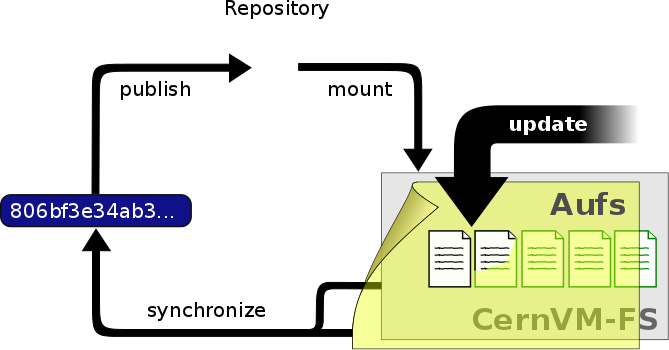
\includegraphics[width=0.8\textwidth]{figures/update_process}
	\end{center}
	\caption{Updating a mounted \cvmfs\ repository by overlaying it with a copy-on-write \aufs\ volume. Any changes will be accumulated in a writable volume (yellow) and can be synchronized into the file catalogs afterwards. The file catalog contains the directory structure as well as file metadata, symbolic links, and secure hash keys of regular files. Regular files are compressed and renamed to their cryptographic content hash before copied into the data store. (NOTE: bitmap will be replaced by vector graphic once I managed to export it)}
	\label{fig:installwebserver}
\end{figure}

\section{Repository Update Procedure}
\label{sct:repoupdate}

Since the repositories may contain many file system objects\footnote{For ATLAS, for example, ``many'' means order of $10^7$ file system objects (\ie number of regular files, symbolic links, and directories).}, we cannot afford to generate an entire repository from scratch for every update.
Instead, we add a writable file system layer on top of a mounted read-only \cvmfs\ repository using an union file system called \aufs~\cite{aufs}.
This renders a usual \cvmfs\ repository writable to the user, while all applied changes are stored in a special writable volume managed by \aufs.
One could see the result as a virtual version of the \emph{shadow tree} we used for updating repositories in previous versions of \cvmfs.
A similar approach is used by Linux Live Distributions that are shipped on read-only media, but allow \emph{virtual} editing of files while running the operating system directly from read-only storage.

If a file in the \cvmfs\ repository gets changed, \aufs\ first copies it to the writable volume and applies any changes to this copy (copy-on-write semantics).
\aufs\ will put newly created files or directories in the writable volume as well.
Additionally it creates special hidden files (called white-outs) to keep track of file deletions in the \cvmfs\ repository.

Eventually, all changes applied to the \emph{virtual shadow tree} are stored in \aufs's writable volume and can be merged into the actual \cvmfs\ repository by a subsequent synchronization step.
This includes compression of new and updated files and updating of the file catalogs.
Before the actual synchronization step takes place, no changes are applied to the \cvmfs\ repository itself.
Therefore, any unsuccessful updates to a repository can be rolled back by simply clearing the writable file system layer of \aufs.

\section{Requirements for a new Repository}
\label{sct:newreporequirements}

In order to create a repository, the server and client part of \cvmfs\ must be installed on your machine.
Furthermore your machine should provide an \aufs\ enabled Kernel as well as a running \texttt{Apache2} web server.
Currently we officially support Scientific Linux 5 and 6 as well as Ubuntu 12.04 distributions.
Please note, that Scientific Linux 6 \emph{does not} ship with an \aufs\ enabled kernel, therefore we provide a compatible patched kernel as an rpm (see Section~\ref{apx:rpms}).

Special care should be taken for the mount location of \cvmfs\ repositories.
From the point of view of the file system, repositories are relocatable.
However, many software installation tools hard-code the full path and therefore break relocatability on the application level.
In effect, repositories have to be mounted at the same location that was used to install it on the release manager machine.
By convention, \cvmfs\ repositories are mounted using their fully qualified repository name under \texttt{/cvmfs}, for instance at \texttt{/cvmfs/atlas.cern.ch}.

\section{\cvmfs\ Repository Creation and Updating}
\label{sct:repocreateandupdate}
To control the server part of \cvmfs\ we provide the versatile \texttt{cvmfs\_server} utility that controls repository creation, updating, deletion, replication and investigation.
Please run it without any parameters to get a short documentation of its commands.

\subsection{Repository Creation}
\label{sct:repocreation}

Given you have successfully installed the \cvmfs\ server part on your machine, you can use \texttt{cvmfs\_server mkfs} to create a fresh repository:\\
\texttt{cvmfs\_server mkfs my.repo.name}
The utility will then ask you for a user that should act as the owner of the repository and afterwards create all the infrastructure for your new \cvmfs\ repository.
Additionally it will create a reasonable default configuration and generate a new release manager certificate and software signing key. You should distribute the public key in \texttt{/etc/cvmfs/keys/my.repo.name} to all your client machines.
Please note, that the \texttt{cvmfs\_server} utility will use \texttt{/srv/cvmfs} as storage location.
In case you want to use a huge hard disk you should mount it there upfront.

When all went fine you should see your repository mounted under \texttt{/cvmfs/my.repo.name} containing only a single file called \texttt{new\_repository}.
Following this step, you can produce the first revision by going through the repository update procedure described in the next Section.

\subsection{Repository Update}
Typically a repository publisher does the following steps in order to create a new revision of a repository:
\begin{enumerate}
	\item Run \texttt{cvmfs\_server transaction} to switch to a copy-on-write enabled \cvmfs\ volume
	\item Make the necessary changes to the repository, \ie add new directories, patch certain binaries, \dots
	\item Test the software installation
	\item Do one of the following:
	\begin{itemize}
		\item Run \texttt{cvmfs\_server publish} and optionally \texttt{cvmfs\_server resign} to finalize your new repository revision \emph{or}
		\item Run \texttt{cvmfs\_server abort} to clear all changes and start over again
	\end{itemize}
	\item Make the web server serve the new version of the repository directory.
\end{enumerate}

Generally \cvmfs\ supports to have more than one repository on a single server machine, but then you need to specify which repository you want to operate on, when running the \texttt{cvmfs\_server} utility commands.
Additionally you should run \texttt{cvmfs\_server resign} every 30 days to update the signatures of the repository.


\include{cpt-details}

%\chapter{Sample Infrastructure Setup}

\appendix
%\include{apx-releasemgr}
\include{apx-rpms}
\chapter{\cvmfs\ Parameters}
\label{apx:parameters}

\section{Client parameters}
Parameters recognized in configuration files under /etc/cvmfs:

\LTXtable{\textwidth}{figures/tabparameters.tex}

\pagebreak

\section{Server parameters}
\LTXtable{\textwidth}{figures/tabserverparameters.tex}


\pagestyle{plain}
\bibliographystyle{alpha}
\bibliography{references}

%\printindex

\end{document}
